%%%%%%%%%%%%%%%%%%%%%%%%%%%%%%%%%%%%%%%%%%%%%%%%%
% Relatório Final - Projeto de Pesquisa
% Métodos de Otimização
% Baltz & Machado
% Capítulo 1
%%%%%%%%%%%%%%%%%%%%%%%%%%%%%%%%%%%%%%%%%%%%%%%%%


\chapter{\Large{Métodos Matemáticos de Otimização}}\label{chp:1}


\section{{O Conceito de Otimização}}

\hspace{0.8cm}
Diz-se otimização, o processo que tem como objetivo encontrar condições que
minimizam ou maximizam algo (seja energia, tempo, dinheiro, etc). Sendo este,
muitas vezes um trabalho árduo, custoso.

Dessa maneira, na matemática, este processo é amplamente utilizado quando
busca-se valores pertencentes ao conjunto \textit{A} (que pode ter
restrições), com o objetivo de encontrar uma solução ótima, aplicando os valores
de \textit{A} em numa função objetivo predefinida.

Podendo assim, ser representada da seguinte forma:

    Dada a função
        \begin{equation}
            f : A \rightarrow \mathbb{R}
        \end{equation}

        \begin{itemize}
                \item Maximização pode ser definida como:
        \end{itemize}

                busca pelo elemento \(x_0 \in A\), que satisfaz:

                    \begin{equation}
                        f(x_0) \geq f(x);
                    \end{equation}

                para todo \(x \in A\).

        \begin{itemize}
                \item Minimização pode ser definida como:
        \end{itemize}

                busca pelo elemento \(x_0 \in A\), que satisfaz:

                    \begin{equation}
                        f(x_0) \leq f(x);
                    \end{equation}

                para todo \(x \in A\).

\vspace{\baselineskip}
Com isso, podemos agora entender como esse processo pode ser custoso. Iniciando
com fato de que existem os pontos máximos e mínimos (pontos críticos), locais
e globais, no espaço das funções. Sendo os pontos críticos locais, aqueles que
não são os menores ou maiores valores para a minimização e maximização,
respectivamente. E os pontos globais, aqueles que representam o menor ou maior
valor no espaço das funções, para a minimização e maximização, respectivamente.

Criando assim, uma certa incerteza ao encontrar um valor crítico numa função,
já que é estritamente difícil saber se o ponto crítico encontrado é local ou
global. Como pode-se perceber na Figura
\ref{grafico_local_global_pontosCriticos}.


\begin{figure}[h]
    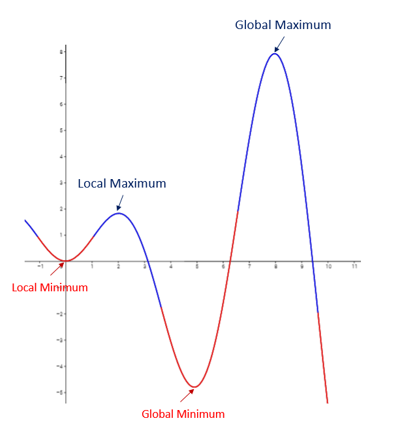
\includegraphics[width=0.43\textwidth]
        {src/grafico_local_global_pontosCriticos.png}
    \centering
    \caption{Exemplo de pontos críticos locais e globais indicados no gráfico
        de uma função}
    \label{grafico_local_global_pontosCriticos}
\end{figure}


\section{{Otimização de Funções à Uma Variável Real}}

\hspace{0.8cm}

Evidente que funções possuem as variáveis dependentes (a qual representa o
objeto da otimização) e variáveis independentes (cujo suas grandezas podem ser
selecionadas), podemos denotar que, para a equação

\begin{equation}
	y = f(x),
\end{equation}
quando buscamos otimizá-la, temos como objetivo encontrar valores que quando
aplicados à \textit{x}, temos o mínimo ou máximo valor \textit{y} (seja ele
local, ou preferencialmente global).

Partindo dessa perspectiva, acaba surgindo a necessidade de utilizar algum
recurso para encontrar o os pontos críticos. E nesse sentindo, pode-se utilizar
a técnica de \textbf{derivação}, donde, oferece como recurso a possibilidade de
identificar tais pontos.

A derivada é a representação da taxa de variação de uma função, em relação a
um ponto. A partir daí, podemos observar um fator interessante; por exemplo,
quando a função está num ponto máximo, existem duas possibilidades, a primeira,
sendo a função parando de crescer e em seguinda se tornando indefinida; e a
segunda possibilidade quando a função para de crescer e começa a decrescer.
Com isso, é importante ressaltar que por definição, quando a derivada (taxa de
variação) em um ponto é positiva, a função cresce, e quando negativa a função
decresce. Conclui-se que, quando a taxa de variação é zero, a função ou para de
crescer ou de decrescer, sendo assim um ponto de máximo ou de mínimo.

Com o uso da derivada, podemos pensar num método de otimização bastante simples,
considerando \(f(x)\) a função que queremos otimizar e \(f'(x)\) sua função
derivada, podemos dizer que o conjunto $O$ possui todos os ótimos locais e
globais de \(f(x)\):

\begin{equation}
    O := \{f(x) | f'(x) = 0\}
\end{equation}


Portanto, aplicando um filtro em $O$ para obeter o máximo e mínimo do conjunto,
acabamos por obeter o máximo e mínimo de \(f(x)\):


\begin{equation}
    max(f(x)) = max(O)
\end{equation}

\begin{equation}
    min(f(x)) = min(O)
\end{equation}


Então podemos perceber dois problemas; determinar como encontrar os pontos onde
a derivada se anule, e determinar se temos de fato todos os pontos.

Considerando por agora, apenas o problema de encontrar os pontos críticos;

Entendendo melhor, a taxa de variação de uma função \(y=f(x)\) em relação a
\(x\), é dada pela relação \(\Delta y / \Delta x\). Sendo esse resultado
correspondente a tangente do ângulo formado pela intersecção entre a reta e a
curva da função \(y\); o coeficiênte ângular da reta à curva.

Sendo o cálculo da taxa de variação demonstrado pela Figura
\ref{derivada_padrao}.

\begin{figure}[h]
    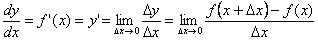
\includegraphics[width=0.45\textwidth]
        {src/derivada_padrao.jpg}
    \centering
    \caption{Derivada: taxa de variação \(dy/dx\).}
    \label{derivada_padrao}
\end{figure}

Partindo desse princípio, é intríseco saber que uma função pode ser derivada
mais de uma vez, sendo essas derivadas, denominadas de `primeira derivada',
`segunda derivada' e por ai em diante. De modo que, a segunda derivada é
a taxa de variação da primeira derivada. Concluindo-se que dada a função
\(f(x)\), sua primeira derivada é \(df/dx = p(x)\), e sua segunda derivada
\(dp/dx = s(x)\).

Considerando que a primeira e segunda derivada são as comunmente utilizadas,
pode-se agora entender a relação entre elas e a função original.

Já sabido que a primeira derivada representa a taxa de variação de um ponto na
curva, a segunda derivada proporciona informações complementares, como por
exemplo, se é um ponto de máximo, mínimo ou inflexão, de modo que ela determina
a concavidade da curva naquele ponto. Como pode-se ver na Figura
\ref{relacao_primeira_segunda_derivada}. E de modo construtivo, é importante
ressaltar que é importante o estudo do gráfico das derivadas de uma função.

\begin{figure}[h]
    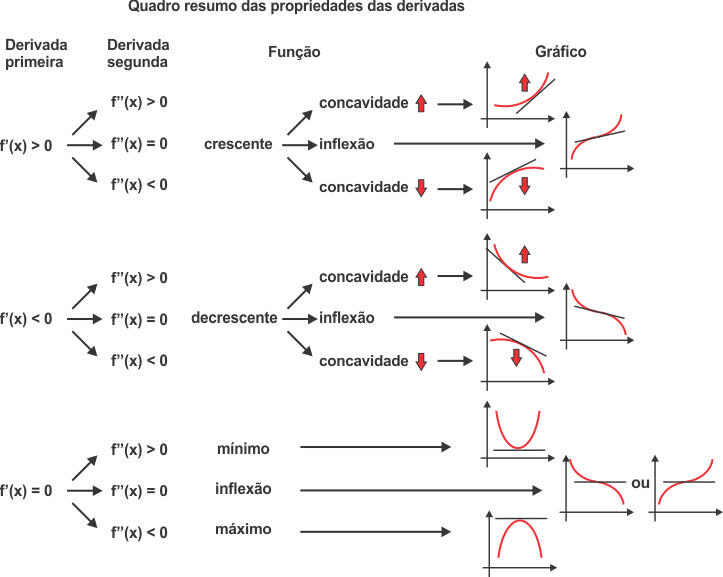
\includegraphics[width=0.65\textwidth]
        {src/relacao_primeira_segunda_derivada.jpg}
    \centering
    \caption{Propriedades e relação da primeira e segunda derivada.}
    \label{relacao_primeira_segunda_derivada}
\end{figure}


\section{{Programando o Método}}

\hspace{0.8cm}


A própria definição da derivada já nos oferece uma uma visão simples de como
ela pode ser implementada num programa de computador. Mas com alguns nuances
que devem ser levados em consideração. Segue a tal implementação:

\begin{lstlisting}[]

pub fn derive1x1_v1<F>(f: &F, x: f64) -> f64
where
    F: Fn(f64) -> f64,
{
    (f(x + h) - f(x)) / h
}


\end{lstlisting}


Essa implementação é ingenua no que se diz respeito a precisão da operação. O
uso depende da aplicação, caso se queira prezar por velocidade de calculo e 
muito pouco sobre precisão, talvez essa solução seja boa o suficiente. O
problema com com precisão desta implementação é que não se é levado em
consideração o aspecto infinitesimal da variação (\(\Delta X\) na figura 1.2, ou
a variável h na implementação em Rust), já que é por este aspecto que
definimos a derivada. Não temos como ter uma variável com tal propriedade num
programa de computador. Como consequência, \(f(x + h) - f(x)\) já é calculada
de forma falha, entregando uma variação diferente da que seria quando se tem
uma variável infinitesimal. O que de fato é entregue é a variação um pouco mais
a frente do ponto esperado.

A partir dai podemos reformular considerando esse deslocamento, redefinindo
da seguinte forma:


\begin{equation}
    f'(x) = \frac{f(x + h) - f(x - h)}{2h}
\end{equation}

Que é equivalente à:

\begin{equation}
    f'(x) = \frac{f(x + h) - f(x - h)}{(x + h) - (x - h)}
\end{equation}


Usaremos essa segunda formulação por motivos de custo de multiplicação de de
números reais se comparado a somas e subtrações, além da possível perca de
precisão. Assim conseguimos compensar o tal deslocamento numa nova função
insignificantemente mais custosa e mais precisa:


\begin{lstlisting}[]

pub fn derive1x1_v2<F>(f: &F, x: f64) -> f64
where
    F: Fn(f64) -> f64,
{
    let x1 = x - h;
    let x2 = x + h;

    let y1 = f(x1);
    let y2 = f(x2);
    return (y2 - y1) / (x2 - x1);
}


\end{lstlisting}






\textcolor[rgb]{1,0,0}{\section{{Otimização de Funções à Várias Variáveis}}}

\hspace{0.8cm}





%
